\documentclass[11pt,a4paper]{article}

\usepackage{notes}

\usepackage{fvextra}
\DefineVerbatimEnvironment{VerbatimWrap}{Verbatim}{breaklines=true}

\title{Greenwich Conduction Task}

\begin{document}

\maketitle
\newpage

\tableofcontents % optional toc
\newpage

\section{Introduction}

\subsection{Purpose}

Documentation explaining the heat conduction differential equation,
the finite difference method used to solve the equation (implemented in C++ code),
and optimizations applied to improve the code's performance.

\subsection{The Heat Equation}

The heat conduction, or \emph{heat diffusion equation}, describes how
heat spreads in a material over time. In two dimensions,
the partial differential heat equation is,
\begin{align}
  \frac{\partial T}{\partial t} =
  k \left(\frac{\partial^2 T}{\partial x^2} +
  \frac{\partial^2 T}{\partial y^2}\right),
\end{align}
where \(k\) is the \emph{thermal diffusivity constant} and
\(T(x,y)\) is the spatial the temperature distribution.

The \emph{steady-state heat equation} is given by:
\begin{align}
  \frac{\partial^2 T}{\partial x^2} + \frac{\partial^2 T}{\partial y^2} = 0
\end{align}
where the heat entering any point is equal to the heat leaving it,
resulting in a stable (or steady) temperature distribution,
i.e., when \(\partial T / \partial t = 0\).

\subsection{Numerical solution using the finite difference method}

The solution to the heat equation
can be approximated with a \emph{finite difference method}.
Finite difference methods discretize the spatial domain,
replacing continuous derivatives with difference quotients.

For a point \((i, j)\) on a 2D grid,
the finite difference approximation of the heat equation can be written as:
\begin{align}
  T_{i,j} = \frac{1}{4}\left(T_{i+1,j} + T_{i-1,j} + T_{i,j+1} + T_{i,j-1}\right)
\end{align}
This formula calculates the temperature \(T_{i,j}\) as the average of
its four neighbouring points. (See Appendix for its derivation).

By iterating this formula across all points in the grid,
we can update each point's temperature until reaching a steady-state solution defined
as some minimum change tolerance.

\subsubsection{Boundary Conditions}

The stated problem uses fixed temperature
values at the boundaries (Dirichlet boundary conditions):
\begin{itemize}
  \item
        \(T(0, y, t) = T_{\text{left}}(y, t)\) = 40°C
  \item
        \(T(L_x, y, t) = T_{\text{right}}(y, t)\) = 90°C
  \item
        \(T(x, 0, t) = T_{\text{bottom}}(x, t)\) = 30°C
  \item
        \(T(x, L_y, t) = T_{\text{top}}(x, t)\) = 50°C
\end{itemize}
These values are set initially and remain constant throughout the simulation.

\newpage
\subsection{Implementation}

\subsubsection{Parameters and setup}

The code takes the following arguments:
\begin{itemize}
  \item
        \texttt{m}: the number of grid points in the \(x\)-direction.
  \item
        \texttt{n}: the number of grid points in the \(y\)-direction.
  \item
        \texttt{tol}: the tolerance level for the maximum temperature difference,
        which serves as the stopping criterion for reaching steady state.
\end{itemize}

The grid \texttt{t} is initialized with dimensions
\((m+2) \times (n+2)\) and filled with an initial temperature of 30°C.
Boundary conditions are then applied based on the specified temperatures.

\subsubsection{Main Iterative Loop}

The main code block implements the following logic:
\begin{enumerate}
  \item
        \emph{Temperature Update}:
        Inside a while loop,
        each internal grid point \(T_{i,j}\)
        is updated according to the finite difference formula.
        The updated temperature values are stored in a separate grid
        \texttt{tnew} to prevent interference
        with the current iteration's calculations.
  \item
        \emph{Convergence Check}:
        The difference between the old and new
        temperatures (\texttt{diff}) is calculated for each point.
        The maximum of these differences (\texttt{difmax}) is tracked.
        Once \texttt{difmax} is smaller than \texttt{tol},
        the loop exits,
        indicating that the solution has converged to a steady state.
  \item
        \emph{Boundary Re-assignment}:
        After updating temperatures,
        \texttt{tnew} values are assigned
        back to \texttt{t} for the next iteration.
\end{enumerate}

\subsubsection{Output}

The code outputs: 
\begin{itemize}
  \item 
  The total number of iterations taken to reach
  convergence. 
  \item 
  The final temperature distribution across the grid,
  including boundary points.
\end{itemize}

\subsubsection{Example usage}

To run the code with a grid of 1000x1000 and a tolerance of 0.01, use:
\begin{verbatim}
build/gauss 1000 1000 0.01
\end{verbatim}

\section{Gauss-Seidel and Jacobi methods}

The two methods,
\emph{Gauss-Seidel} and \emph{Jacobi},
are iterative techniques used to solve partial
differential equations like the heat equation by
approximating values on a grid.
Both methods calculate a steady-state temperature
distribution across the grid but update calculations differently.
Below, we discuss the key differences
between the Gauss-Seidel and Jacobi methods in the provided codes.

\subsection{Gauss-Seidel Method}

The Gauss-Seidel method updates each grid point's temperature in place,
meaning it immediately uses the most recent values within the same
iteration.
This can lead to faster convergence because each calculation
benefits from the latest available information.

\subsubsection{Key Characteristics}

\begin{itemize}
  \item
        \emph{In-Place Update}:
        When calculating the new temperature for \(T_{i,j}\),
        the Gauss-Seidel method immediately updates the
        temperature in the original grid \texttt{t}.
  \item
        \emph{Fast Convergence}:
        Since the latest values are used immediately,
        convergence generally occurs faster than with the Jacobi method.
  \item
        \emph{Implementation}:

        \begin{itemize}
          \item
                The updated values are written directly back into \texttt{t}.
          \item
                The maximum difference \texttt{difmax} is calculated within the same
                loop where \texttt{t[i][j]} is updated.
        \end{itemize}
\end{itemize}

\subsubsection{Code Snippet (Gauss-Seidel)}

Here's a snippet illustrating the Gauss-Seidel approach:

\begin{VerbatimWrap}
for (int i = 1; i <= m; i++) {
  for (int j = 1; j <= n; j++) {
      tnew[i][j] = (t[i-1][j] + t[i+1][j] + t[i][j-1] + t[i][j+1]) / 4.0;
      diff = std::fabs(tnew[i][j] - t[i][j]);
      if (diff > difmax) {
          difmax = diff;
      }
      t[i][j] = tnew[i][j]; // immediate in-place update
  }
}  
\end{VerbatimWrap}

\subsection{Jacobi Method}

The Jacobi method calculates all updated values for the grid in a
separate matrix (\texttt{tnew}) and only transfers these values to the
main grid (\texttt{t}) once the entire grid has been processed. 
This can be more computationally expensive since it doesn't benefit from the latest updates in the current iteration, leading to a slower
convergence.

\subsubsection{Key Characteristics}

\begin{itemize}
\item
  \emph{Separate Grid Update}: 
  Each point's updated temperature is
  stored in \texttt{tnew}, and \texttt{t} is only updated at the end  of each iteration.
\item
  \emph{Slower Convergence}: 
  Because it uses only the previous iteration's values, 
  convergence is slower than in Gauss-Seidel.
\item
  \emph{Implementation}:
  \begin{itemize}
  \item
    The update for \texttt{tnew[i][j]} is done in one loop.
  \item
    A second loop copies values from \texttt{tnew} to \texttt{t} and
    calculates \texttt{difmax}.
  \end{itemize}
\end{itemize}

\subsubsection{Code Snippet (Jacobi)}

In the Jacobi code, updates and copying are separated:
\begin{VerbatimWrap}
for (int i = 1; i <= m; i++) {
    for (int j = 1; j <= n; j++) {
        tnew[i][j] = (t[i-1][j] + t[i+1][j] + t[i][j-1] + t[i][j+1]) / 4.0;
    }
}

for (int i = 1; i <= m; i++) {
    for (int j = 1; j <= n; j++) {
        diff = std::fabs(tnew[i][j] - t[i][j]);
        if (diff > difmax) {
            difmax = diff;
        }
        t[i][j] = tnew[i][j]; // copy tnew to t at the end of each iteration
    }
}
\end{VerbatimWrap}

\subsection{Summary of differences}

The \emph{Gauss-Seidel method} generally converges faster than
\emph{Jacobi} due to its in-place update mechanism, 
which leverages the latest information during calculations. 
However, the Jacobi method is easier to parallelize since each update only depends on values from
the previous iteration, 
making it more suitable for certain parallel
computing environments. 
Both methods ultimately reach the same
steady-state solution for the heat conduction problem, but Gauss-Seidel
is typically more computationally efficient in sequential
implementations.

\section{Results}

\subsection{Hardware}

All following calculations are run on a Dell Core i5 with 4 cores.

\subsection{Benchmark}

We run the C++ code on a grid of 1000x1000 with a tolerance of 0.01.
Figure \ref{fig:temp-distro} plots the result.

\begin{figure}[!htb]
  \centering
  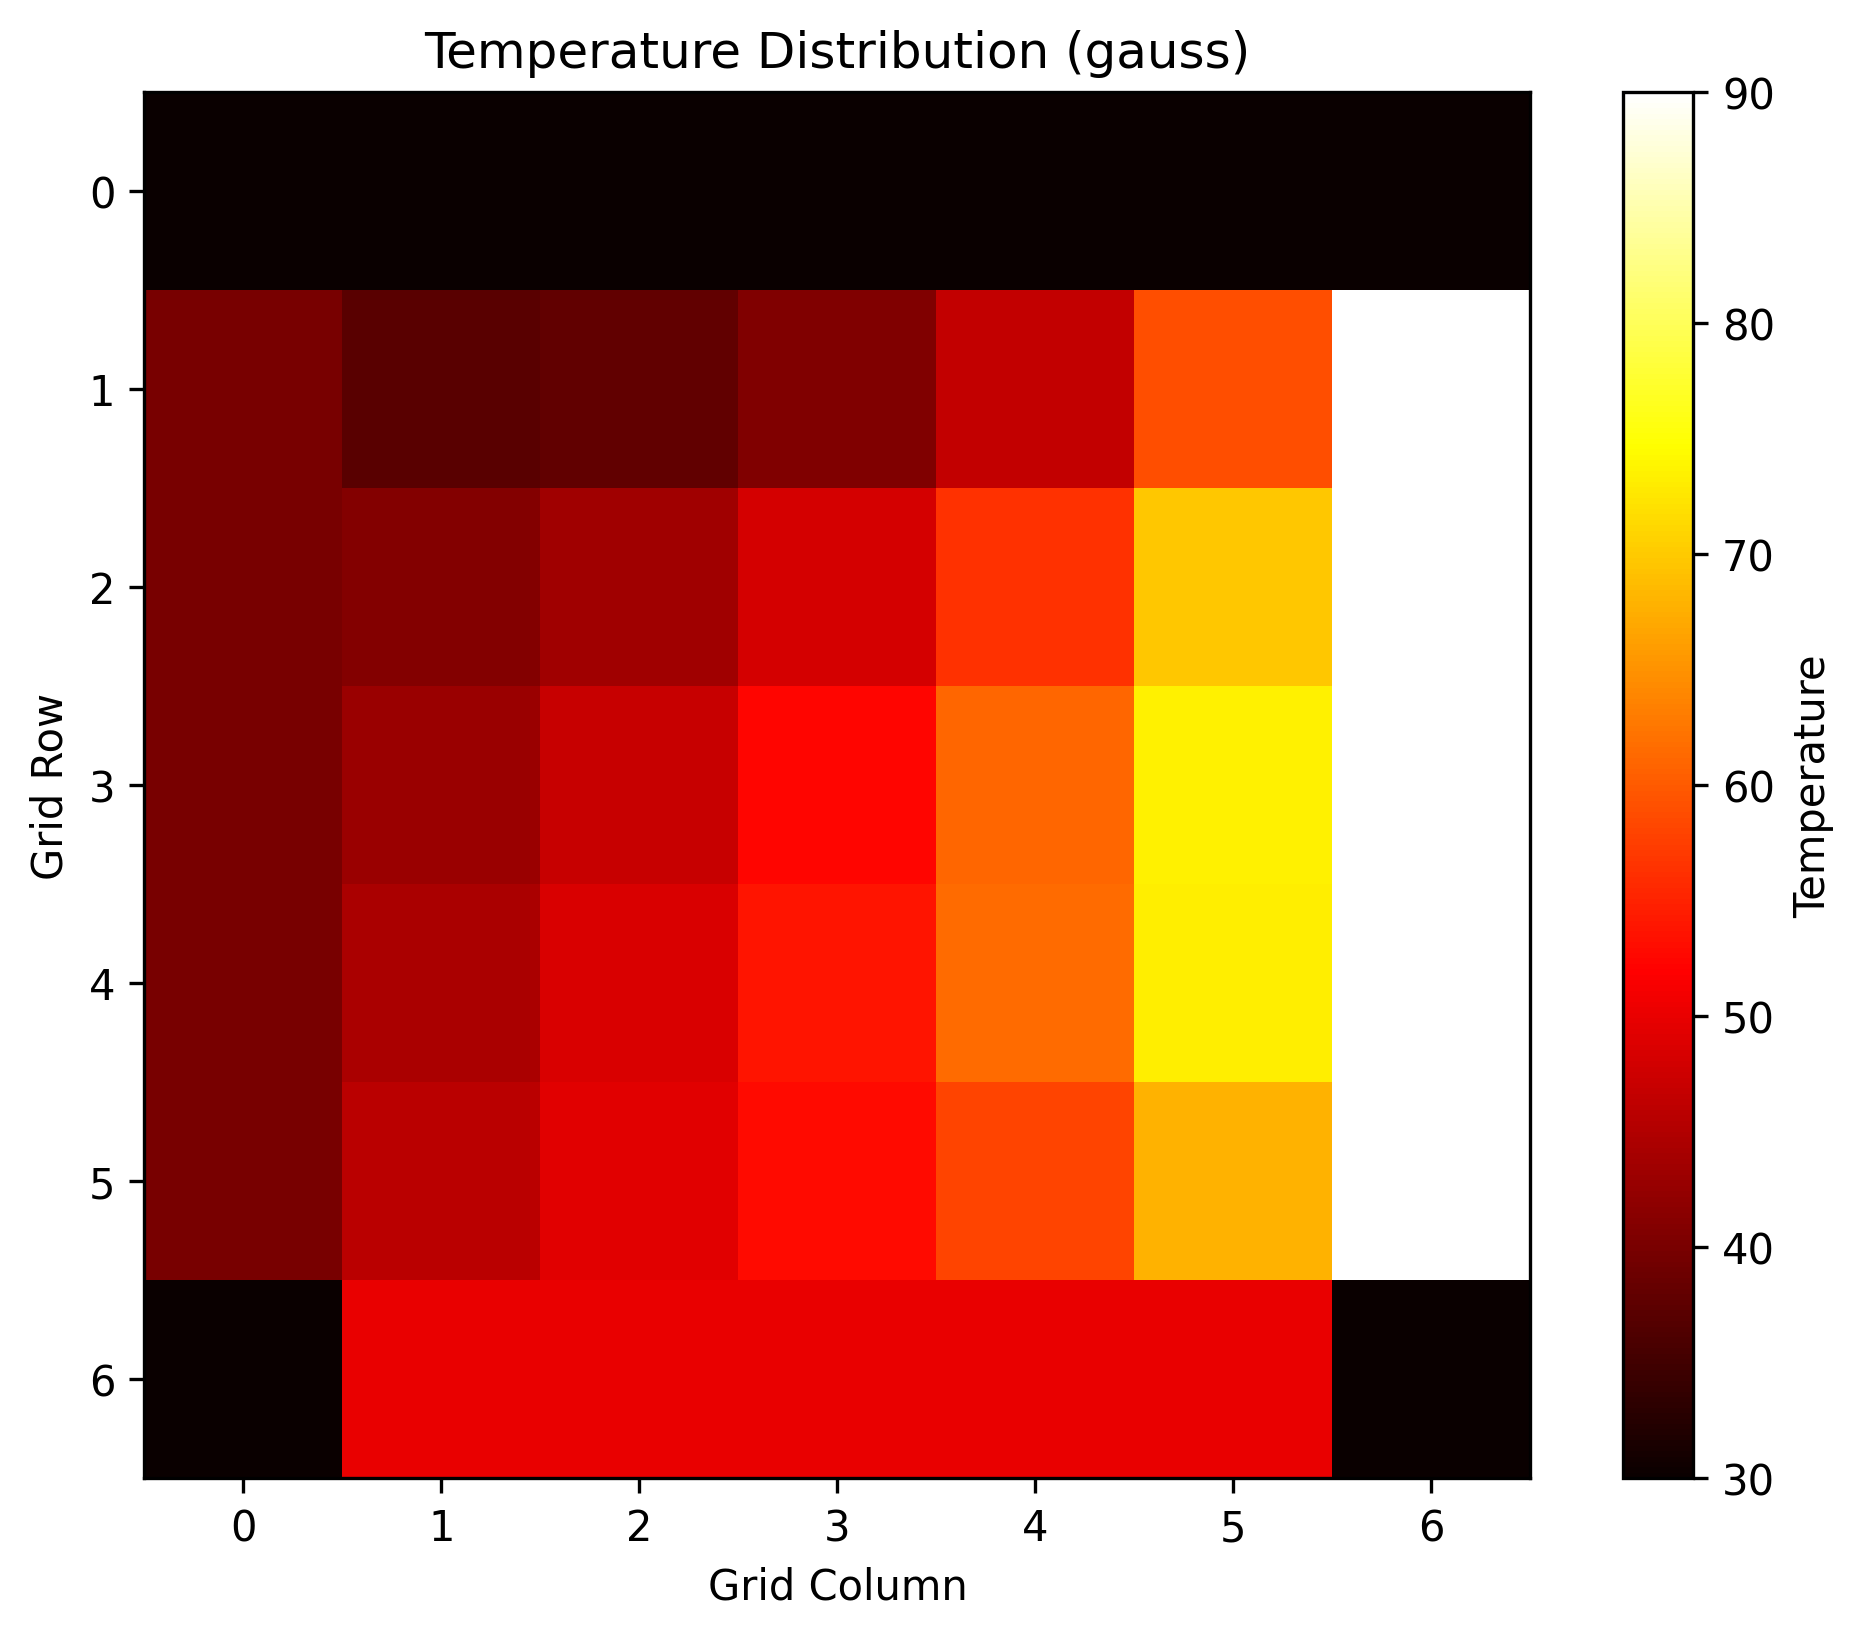
\includegraphics[width=0.7\linewidth]{../results/plots/temperature_distribution_gauss.png}
  \caption{Steady state temperature distribution on a 1000x1000 grid with 
  tolerance 0.01 using the Gauss-Seidel method.}
  \label{fig:temp-distro}
\end{figure}

Comparison of run times shows that the execution of the Gauss-Seidel method takes 72 seconds compared to the Jacobi method that takes 79 seconds in agreement with the summary in the previous section.

\subsection{Optimization}

We now apply parallelization to speed up calculations for the two methods.
We focus on OpenMP (Open Multi-Processing), 
an application programming interface (API) that supports multi-platform shared-memory parallel programming in C, C++, and Fortran. 
OpenMP enables developers to write code that can run in parallel across multiple CPU cores, 
effectively allowing tasks to be divided and processed simultaneously.

\subsubsection{Parallelizing the Jacobi Method}

Since the Jacobi method uses a separate grid (\texttt{tnew}), 
updates for each grid point only depend on values from the previous iteration.
OpenMP can parallelize the nested loops used to update grid points. 
Here’s an example:

\begin{VerbatimWrap}
// Update temperature for next iteration in parallel
#pragma omp parallel for
for (int i = 1; i <= m; i++)
{
    for (int j = 1; j <= n; j++)
    {
        tnew[i][j] = (t[i - 1][j] + t[i + 1][j] + t[i][j - 1] + t[i][j + 1]) / 4.0;
    }
}
\end{VerbatimWrap}

\subsubsection{Parallelizing the Gauss-Seidel method}

The Gauss-Seidel method requires each point to use the most recent values, 
making it harder to parallelize than the Jacobi method.
The outer loop time loop can be parallelized, 
which updates the temperature and calculates the maximum difference. 
This allows each iteration to be executed concurrently across multiple threads.

\begin{VerbatimWrap}
// Update temperature and calculate maximum difference
#pragma omp parallel for reduction(max : difmax) private(diff)
for (int i = 1; i <= m; i++)
{
    for (int j = 1; j <= n; j++)
    {
        tnew[i][j] = (t[i - 1][j] + t[i + 1][j] + t[i][j - 1] + t[i][j + 1]) / 4.0;

        // Calculate difference and update difmax in a thread-safe manner
        diff = std::fabs(tnew[i][j] - t[i][j]);
        if (diff > difmax)
        {
            difmax = diff;
        }

        // Copy new value to old temperature array
        t[i][j] = tnew[i][j];
    }
}
\end{VerbatimWrap}

\subsubsection{Implementation}

When using libraries like OpenMP, 
it's important to compile the code with the \texttt{-fopenmp} flag:

\begin{VerbatimWrap}
  g++ -fopenmp parallel/gauss.cpp -o build/gauss
\end{VerbatimWrap}

\subsubsection{Comparison of runtimes}

Applying parallelization roughly halves the run times for both algorithms.
The Gauss-Seidel method benefits from parallelization with a runtime reduction from 
72.7995 seconds to 42.1727 seconds.
The Jacobi method benefits from parallelization with a runtime reduction from 
79.0255 seconds to 39.1713 seconds.

\newpage
\section{Appendix}

The heat equation in two dimensions is given by:
\begin{equation}
  \frac{\partial T}{\partial t} =
  k \left( \frac{\partial^2 T}{\partial x^2} +
  \frac{\partial^2 T}{\partial y^2} \right)
\end{equation}
where \(T\) is the temperature, \(t\) is time,
\(k\) is the thermal diffusivity,
and \(x\) and \(y\) are spatial dimensions.

To solve this equation numerically,
we discretize the spatial domain into a grid with points \((i, j)\),
where: \(i\) corresponds to the index in the \(x\)-direction,
and \(j\) corresponds to the index in the \(y\)-direction.
We denote the temperature at point \((i, j)\) as \(T_{i,j}\).

Next, replace the continuous derivatives with finite differences.
The second spatial derivatives can be approximated using central difference formulas:
\begin{align}
  \frac{\partial^2 T}{\partial x^2} \approx
  \frac{T_{i+1,j} - 2T_{i,j} + T_{i-1,j}}{\Delta x^2},
\end{align}
and,
\begin{align}
  \frac{\partial^2 T}{\partial y^2} \approx
  \frac{T_{i,j+1} - 2T_{i,j} + T_{i,j-1}}{\Delta y^2}.
\end{align}
where \(\Delta x\) and \(\Delta y\) are the grid spacings in the \(x\) and \(y\) directions,
respectively.

Substituting the finite difference approximations into the heat equation gives us:
\begin{align}
  \frac{\partial T_{i,j}}{\partial t} =
  k \left( \frac{T_{i+1,j} - 2T_{i,j} +
    T_{i-1,j}}{\Delta x^2} +
  \frac{T_{i,j+1} - 2T_{i,j} + T_{i,j-1}}{\Delta y^2} \right).
\end{align}
Assuming uniform grid spacing (\( \Delta x = \Delta y = \Delta \)) yields:
\begin{align}\label{eq:discrete-conduction-space}
  \frac{\partial T_{i,j}}{\partial t} =
  k \left( \frac{T_{i+1,j} -
    2T_{i,j} + T_{i-1,j}}{\Delta^2} +
  \frac{T_{i,j+1} - 2T_{i,j} + T_{i,j-1}}{\Delta^2} \right)
\end{align}
Next,
we use an explicit time-stepping method (like Euler’s method) to discretize time.
We denote the temperature at the next time step as \(T^{n+1}_{i,j}\),
and at the current time step as \(T^n_{i,j}\) so that:
\begin{align}
  T^{n+1}_{i,j} = T^n_{i,j} +
  \Delta t \cdot \frac{\partial T_{i,j}}{\partial t}
\end{align}
Substituting this into equation \ref{eq:discrete-conduction-space} gives:
\begin{align}\label{eq:discrete-conduction-spacetime}
  T^{n+1}_{i,j} & =
  T^n_{i,j} +
  k \Delta t \left( \frac{T^{n}_{i+1,j} - 2T^{n}_{i,j} +
    T^{n}_{i-1,j}}{\Delta^2} + \frac{T^{n}_{i,j+1} - 2T^{n}_{i,j} +
    T^{n}_{i,j-1}}{\Delta^2} \right)
\end{align}
For large \(n\),
the solution approaches a steady-state where \( T^{n+1}_{i,j} = T^{n}_{i,j} \).
Again,
substituting this into equation \ref{eq:discrete-conduction-spacetime} yields:
\begin{equation}
  T_{i,j} = \frac{1}{4}\left(T_{i+1,j} + T_{i-1,j} + T_{i,j+1} + T_{i,j-1}\right).
\end{equation}

\end{document}